\documentclass[border=2pt]{standalone}
\usepackage{pgfplots}
\pgfplotsset{compat=1.18}
\begin{document}
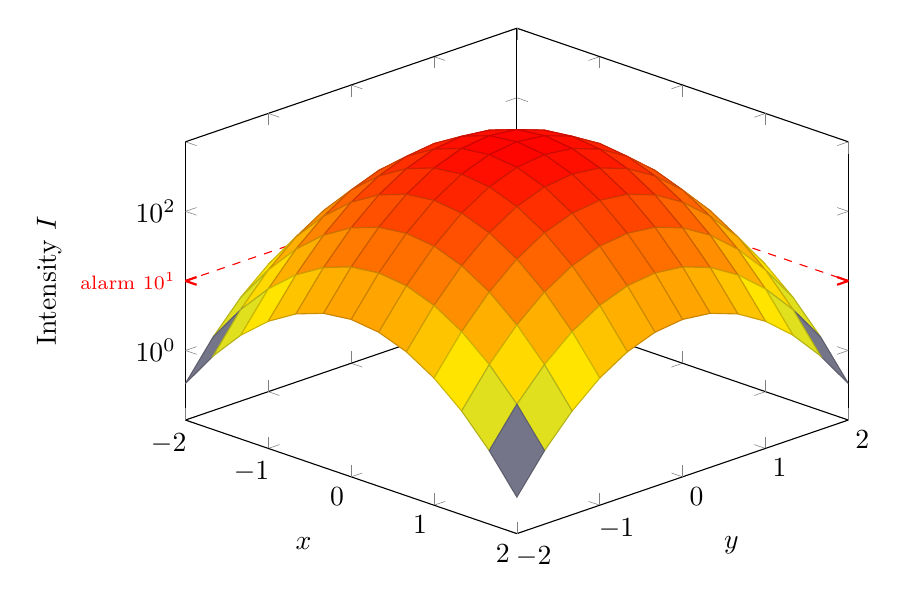
\begin{tikzpicture}
  \begin{axis}[
    width=10cm,
    height=8cm,
    view={45}{30},
    domain=-2:2,
    y domain=-2:2,
    samples=13,
    zmode=log,
    zmin=0.1,
    zmax=1000,
    grid=none,
    xlabel={$x$},
    ylabel={$y$},
    zlabel={Intensity $I$},
    extra z ticks={10},
    extra z tick labels={alarm $10^1$},
    extra z tick style={grid=major,grid style={red,dashed},tick style={red,line width=0.8pt},tick label style={text=red,font=\scriptsize}}
  ]
    \addplot3[surf] {1000*exp(-(x*x+y*y))};
  \end{axis}
\end{tikzpicture}
\end{document}
